\title{Warm-Up for March 7th, 2022}
\author{Dr. Jordan Hanson - Whittier College Dept. of Physics and Astronomy}
\date{\today}
\documentclass[12pt]{article}
\usepackage[a4paper, total={18cm, 27cm}]{geometry}
\usepackage{graphicx}
\usepackage{amsmath}
\usepackage{bm}
\begin{document}
\maketitle

\section{Memory Bank}

\begin{enumerate}
\item In two dimensions, solutions to the Laplacian at coordinates $(x,y)$ are equal to the average value on a circle of radius $R$ centered around $(x,y)$:
\begin{equation}
V_{\rm ave} = V(x,y) = \frac{1}{2\pi R}\oint_{\rm circle} V dl \label{eq:ave}
\end{equation}
\item Obtaining voltage from field: $V(\mathbf{r}) = - \int_{\mathcal{O}}^{\mathbf{r}} \mathbf{E} \cdot d\mathbf{l}$
\end{enumerate}

\section{Solutions to the Laplacian for Potential}

\begin{enumerate}
\item Consider the following function of $s$ in cylindrical coordinates:
\begin{equation}
V(s) = V_0 \left(\frac{\sin(s)}{s}\right) \label{eq:V}
\end{equation}
Note that $V(0) = V_0$.  Using Eq. \ref{eq:ave}, calculate the average value of $V(s)$ on a circle of radius $R = \pi$, centered on $s = 0$.  Remark on the viability of Eq. \ref{eq:V} as a solution to Laplace's equation. \\ \vspace{2cm}
\item Recall the example of the neutral coaxial cable from the homework (Fig. \ref{fig:coax}). (a) Use Gauss' law to find the field $\mathbf{E}$ for $a < s < b$ in cylindrical coordinates. (b) Integrate the field to find the potential for $a < s < b$. (c) Following Eq. \ref{eq:ave}, compute the average potential over a circle of radius $s = a$.  Does Eq. \ref{eq:ave} hold?  Why or why not?
\end{enumerate}

\begin{figure}
\centering
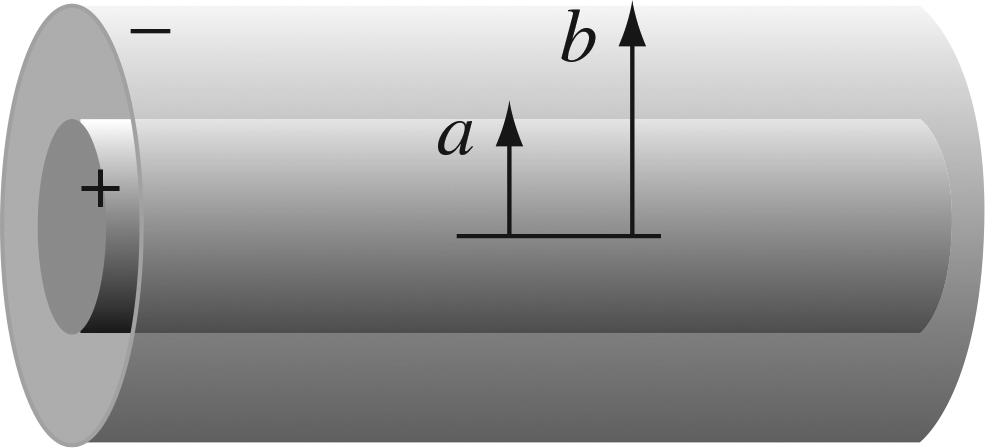
\includegraphics[width=0.3\textwidth]{figures/2_26.jpg}
\caption{\label{fig:coax} Figure 2.26 from the text, depicting a model for a neutral coaxial cable with static charge.}
\end{figure}

\end{document}